\section{Diferencia entre maquinas virtuales y contenedores} 
El objetivo principal de estas tecnologias, es la de dar un entorno de desarrollo con ciertas caracteristicas por lo que parecen estas tecnologias, maquinas virtuales y contenedores, donde la primera es una copia exacta del software y hardware, en cambio los contenedores no hay una copia si no que tienen los archivos necesarios para poder correr un determinado software.

\begin{itemize}
	\item Jerarquia maquina virtual
	\\La primer gran diferencia es la jerarquia, forma de como estan constituidas. En el primero de los casos las maquinas virtuales estan constituidas por:
	\\ \textbf{-El servidor o una computador}.
	\\ \textbf{-El sistema operativo} que hospeda y administra los recursos del servidor o computador.
	\\ \textbf{-El hypervisor} plataforma que monitoriea y controlas virtualizacion.
	\\ \textbf{-Sistema virtualizado} sistema operativo que fue virtualizado (copia total de software y hardware).
	\\ \textbf{-Bins/Libs} Binarios y librerias.
	\\ \textbf{-App} Aplicacion a ejecutar.
	\begin{center}
	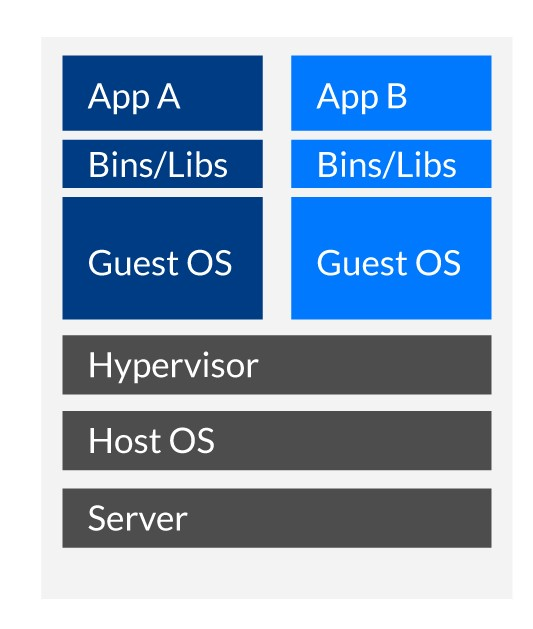
\includegraphics[width=8cm]{./Imagenes/jerarquia1} 
	\end{center}

\end{itemize} 


\begin{itemize}
	\item Jerarquia contenedor
	\\ \textbf{-El servidor o una computador}.
	\\ \textbf{-El sistema operativo} que hospeda y administra los recursos del servidor o computador.
	\\ \textbf{-Docker Engine} virtualizacion a nivel del sistema operativo permite multiples instancias aisladas.
	\\ \textbf{-Bins/Libs} Binarios y librerias.
	\\ \textbf{-App} Aplicacion a ejecutar.
	\begin{center}
	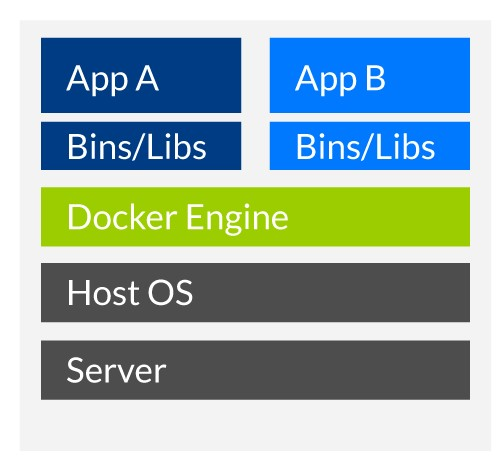
\includegraphics[width=8cm]{./Imagenes/jerarquia2} 
	\end{center}
\end{itemize} 

\begin{itemize}
	\item Los contenedores permiten desplegar aplicaciones más rápido, arrancarlas y pararlas más rápido y aprovechar mejor los recursos de hardware.
	\item La solución de virtualización permite gestionar de forma centralizada los sistemas virtualizados así como sus recursos de almacenamiento:
	\item Reducción de los costes de IT gracias al aumento de la eficiencia y la flexibilidad en el uso de recursos.
	\item Administración global centralizada y simplificada.
	\item Mejora en los procesos de clonación y copia de sistemas: Mayor facilidad para la creación de entornos de test que permiten poner en marcha nuevas aplicaciones sin impactar a la producción, agilizando el proceso de las pruebas.
	\item Aislamiento : un fallo general de sistema de una máquina virtual no afecta al resto de máquinas virtuales.



\end{itemize} 